\PassOptionsToPackage{svgnames}{xcolor}
\documentclass[t, english]{beamer}
\usepackage[utf8]{inputenc}
\usepackage[T1]{fontenc}
\usepackage{tikz}
\usepackage{LobsterTwo}
\usepackage[default]{comfortaa}
\usepackage{pgfpages}
\usepackage{listings}
\usepackage{appendixnumberbeamer}
\lstset{
  basicstyle=\ttfamily\scriptsize\color{black},
  showstringspaces=false,
  commentstyle=\color{red},
  keywordstyle=\color{blue},
  language=bash,
  backgroundcolor=\color{black},
}
%\pgfpagesuselayout{8 on 1}[a4paper, border shrink=5mm]
%\setbeameroption{show notes on second screen=bottom}
\setbeameroption{hide notes}
%\setbeameroption{show notes}
\setbeamertemplate{note page}[plain]
\beamertemplatenavigationsymbolsempty
\synctex=1
\hypersetup{pdfpagemode=UseNone} % don't show bookmarks on initial view
\usetheme{default}
%\usefonttheme{professionalfonts}
\setbeamertemplate{footline}{%
\raisebox{5pt}{%
\makebox[\paperwidth]{%
\hfill\makebox[25pt]{%
\scriptsize\insertframenumber/\inserttotalframenumber%
}%
}%
}\hspace*{5pt}%
}
% http://www.texample.net/tikz/examples/hand-drawn-lines/
\usetikzlibrary{calc,decorations.pathmorphing,patterns,trees}
\pgfdeclaredecoration{penciline}{initial}{
\state{initial}[width=+\pgfdecoratedinputsegmentremainingdistance,
auto corner on length=1mm,]{
\pgfpathcurveto%
{% From
\pgfqpoint{\pgfdecoratedinputsegmentremainingdistance}
{\pgfdecorationsegmentamplitude}
}
{% Control 1
\pgfmathrand
\pgfpointadd{\pgfqpoint{\pgfdecoratedinputsegmentremainingdistance}{0pt}}
{\pgfqpoint{-\pgfdecorationsegmentaspect
\pgfdecoratedinputsegmentremainingdistance}%
{\pgfmathresult\pgfdecorationsegmentamplitude}
}
}
{%TO
\pgfpointadd{\pgfpointdecoratedinputsegmentlast}{\pgfpoint{1pt}{1pt}}
}
}
\state{final}{}
}
\tikzset{
photo/.style= {
rectangle,
line width=8pt,
draw=DarkGreen,
decorate,
decoration={penciline},
inner sep=0pt
}
}
\input Konanur.fd
\newcommand*\initfamily{\usefont{U}{Konanur}{xl}{n}}
% http://tex.stackexchange.com/questions/16964/block-quote-with-big-quotation-marks
\newcommand*\quotesize{60}
\newcommand*{\openquote}
{\tikz[remember picture,overlay,xshift=-4ex,yshift=-1ex]
\node (OQ) {\fontsize{\quotesize}{\quotesize}\selectfont``};\kern0pt}
\newcommand*{\closequote}
{\tikz[remember picture,overlay,xshift=4ex,yshift=-4ex]
\node (CQ) {\fontsize{\quotesize}{\quotesize}\selectfont''};}
\newenvironment{shadequote}[4]%
{%
\begin{minipage}{.25\textwidth}
\noindent
\includegraphics[width=\textwidth]{#4}\\
{\scriptsize\bfseries\itshape #1}
\\
{\tiny #2 \newline at #3}
\end{minipage}
\hfill
\begin{minipage}[c]{.7\textwidth}
\LobsterTwo
%\begin{cursive}
\begin{quote}\openquote{}
}%
{%
\hfill\closequote{}\end{quote}
%\end{cursive}
\end{minipage}
}


\begin{document}

\title{Etude et réalisation du serveur de la nouvelle plate-forme CosyVerif}
\author{Idrissa SOKHONA}
\date{29 Septembre 2014}

\LobsterTwo

\begin{frame}
\begin{center}

\par
\Huge Etude et réalisation du serveur de la nouvelle plate-forme CosyVerif

\par
\normalsize
\textsf{Idrissa SOKHONA}

\par
\textsf{idrissa.sokhona@etu.upmc.fr}

\par
\textsf{Université Pierre et Marie Curie,}

\par
\textsf{Master informatique,}

\par
\textsf{Spécialité SAR, Parcours SRETR}

\begin{tikzpicture}
    \node
      [anchor=north]
      at (1,3)
      {
\includegraphics[height=2cm]{img/lipn}};
    \node
      [anchor=north]
      at (6.5,3)
      {
\includegraphics[height=2cm]{img/lsv}};
  \end{tikzpicture}
\end{center}
\end{frame}

\begin{frame}[c]
  \frametitle{Context}
  
  \begin{minipage}{1\textwidth}
  	\only <1>{%
                \begin{tikzpicture}
                      \node
                          [anchor=north]
                          at (0,0)
                          {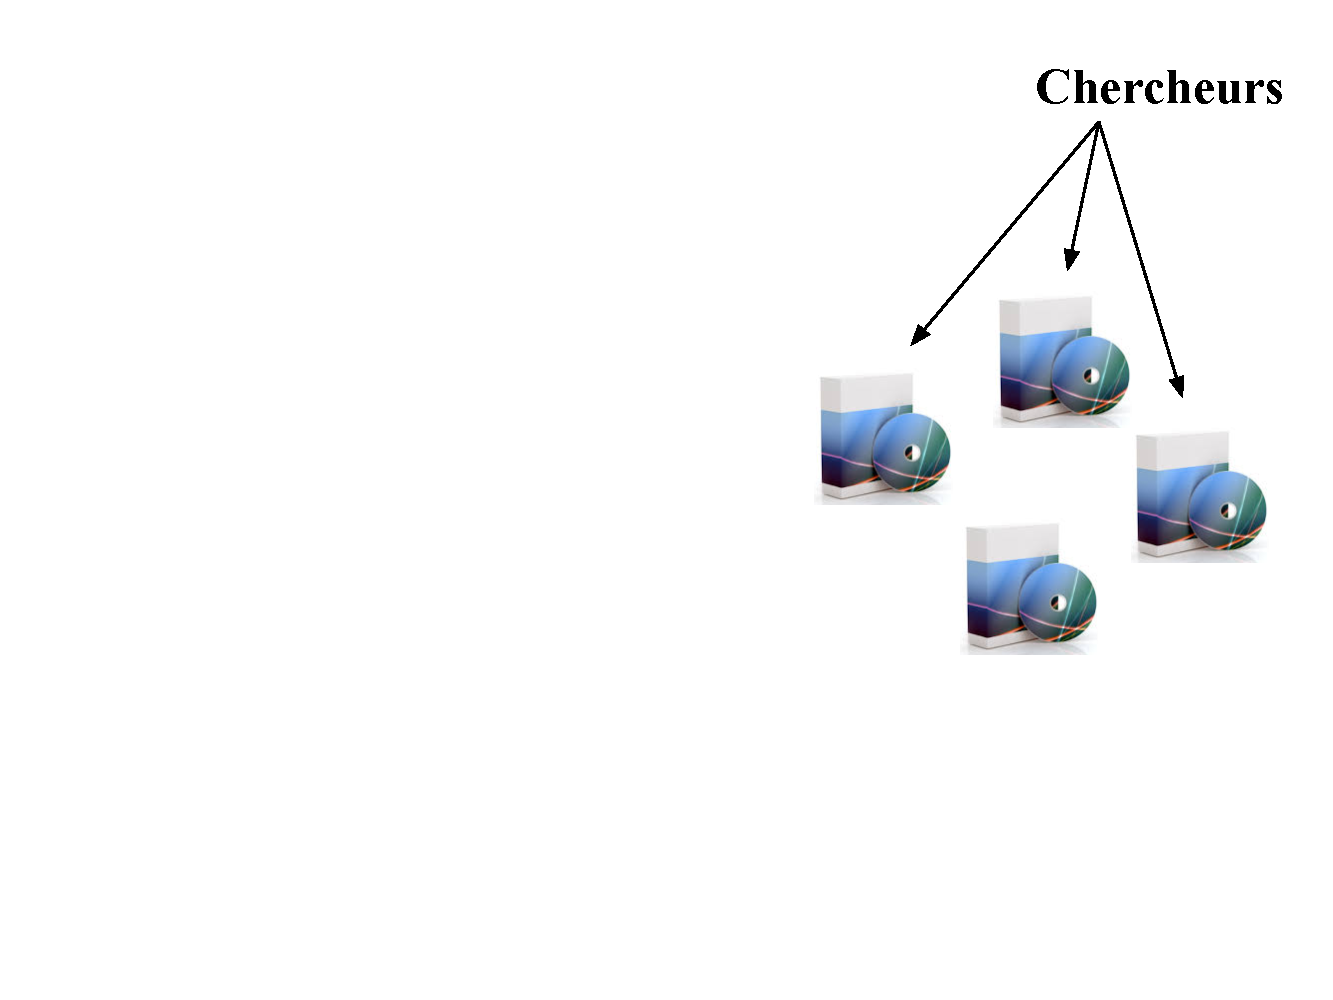
\includegraphics[width=10.5cm, height=4cm]{img/1-chercheur}};
                 \end{tikzpicture}
            }%
            
            \only <2-7>{%
                \begin{tikzpicture}
                      \node
                          [anchor=north]
                          at (0,0)
                          {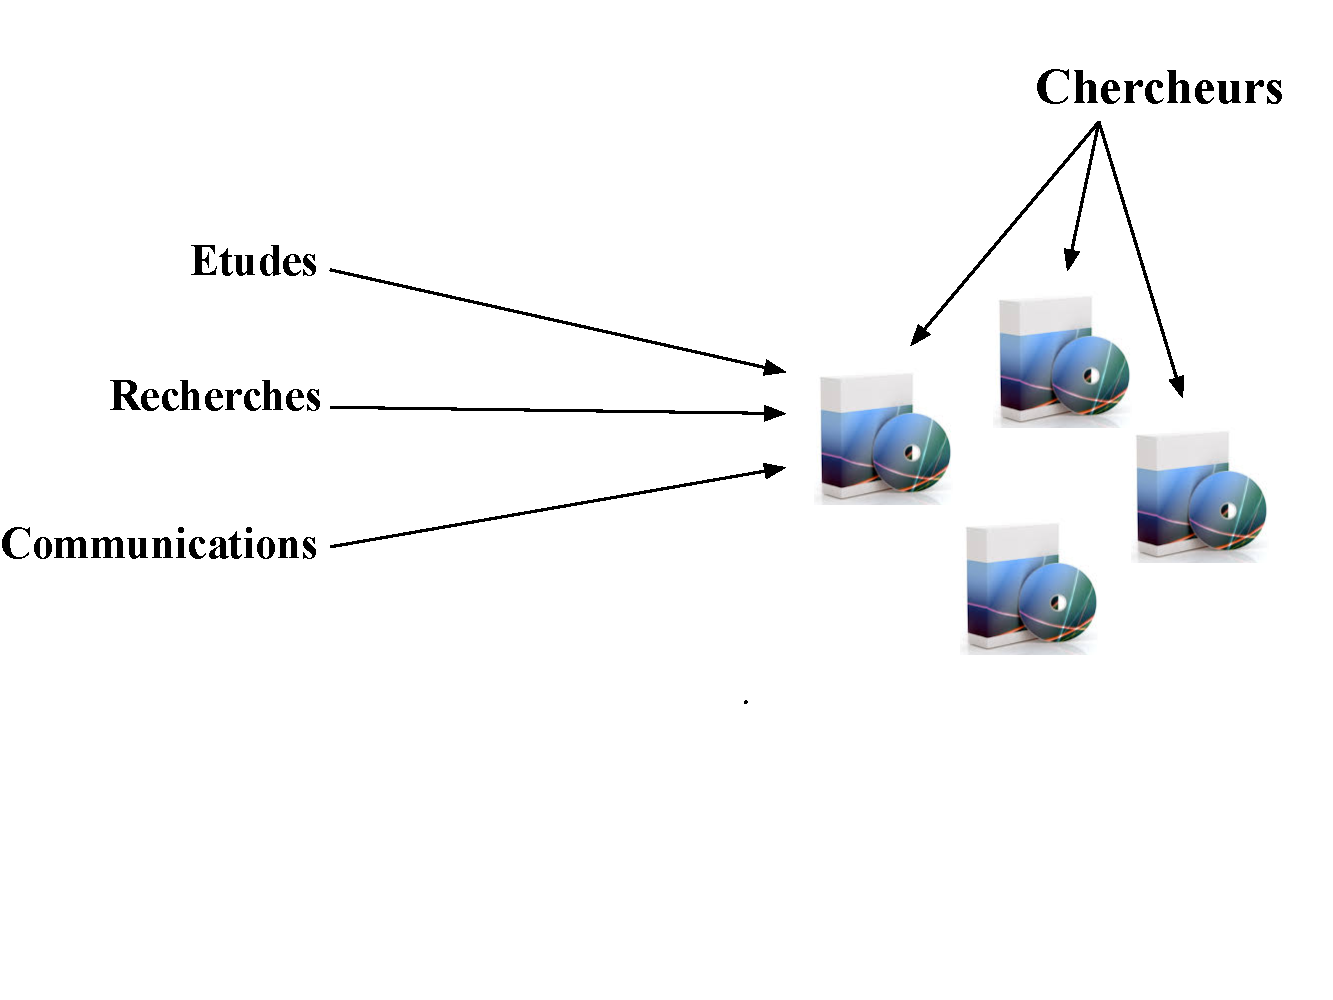
\includegraphics[width=10.5cm, height=4cm]{img/2-chercheur}};
                 \end{tikzpicture}
            }%
            
            \only <8>{%
                \begin{tikzpicture}
                      \node
                          [anchor=north]
                          at (0,0)
                          {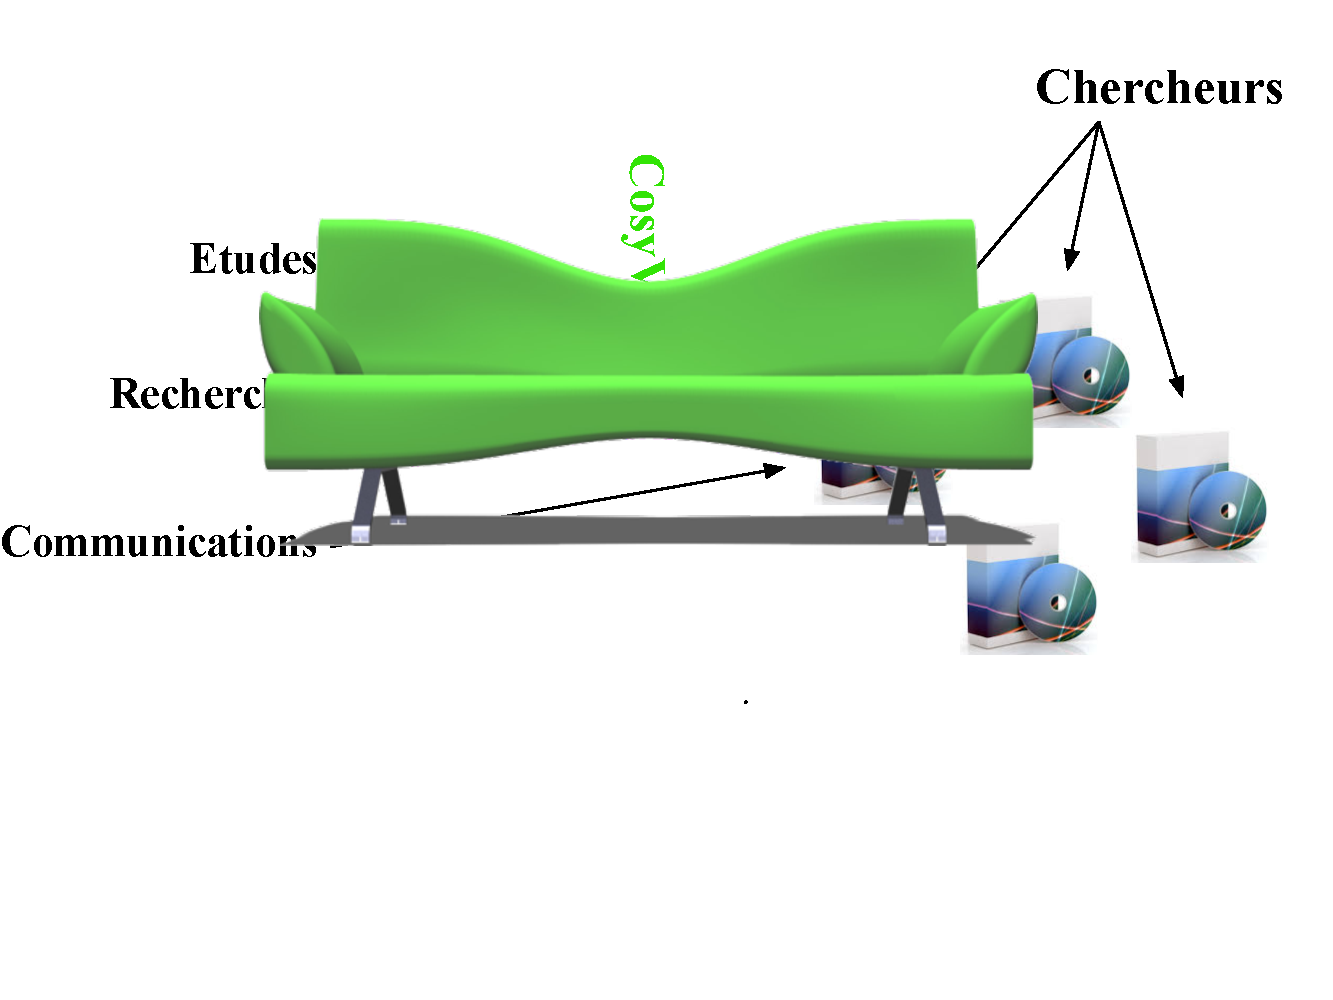
\includegraphics[width=10.5cm, height=4cm]{img/3-chercheur}};
                 \end{tikzpicture}
            }%
            
            \only <9>{%
                \begin{tikzpicture}
                      \node
                          [anchor=north]
                          at (0,0)
                          {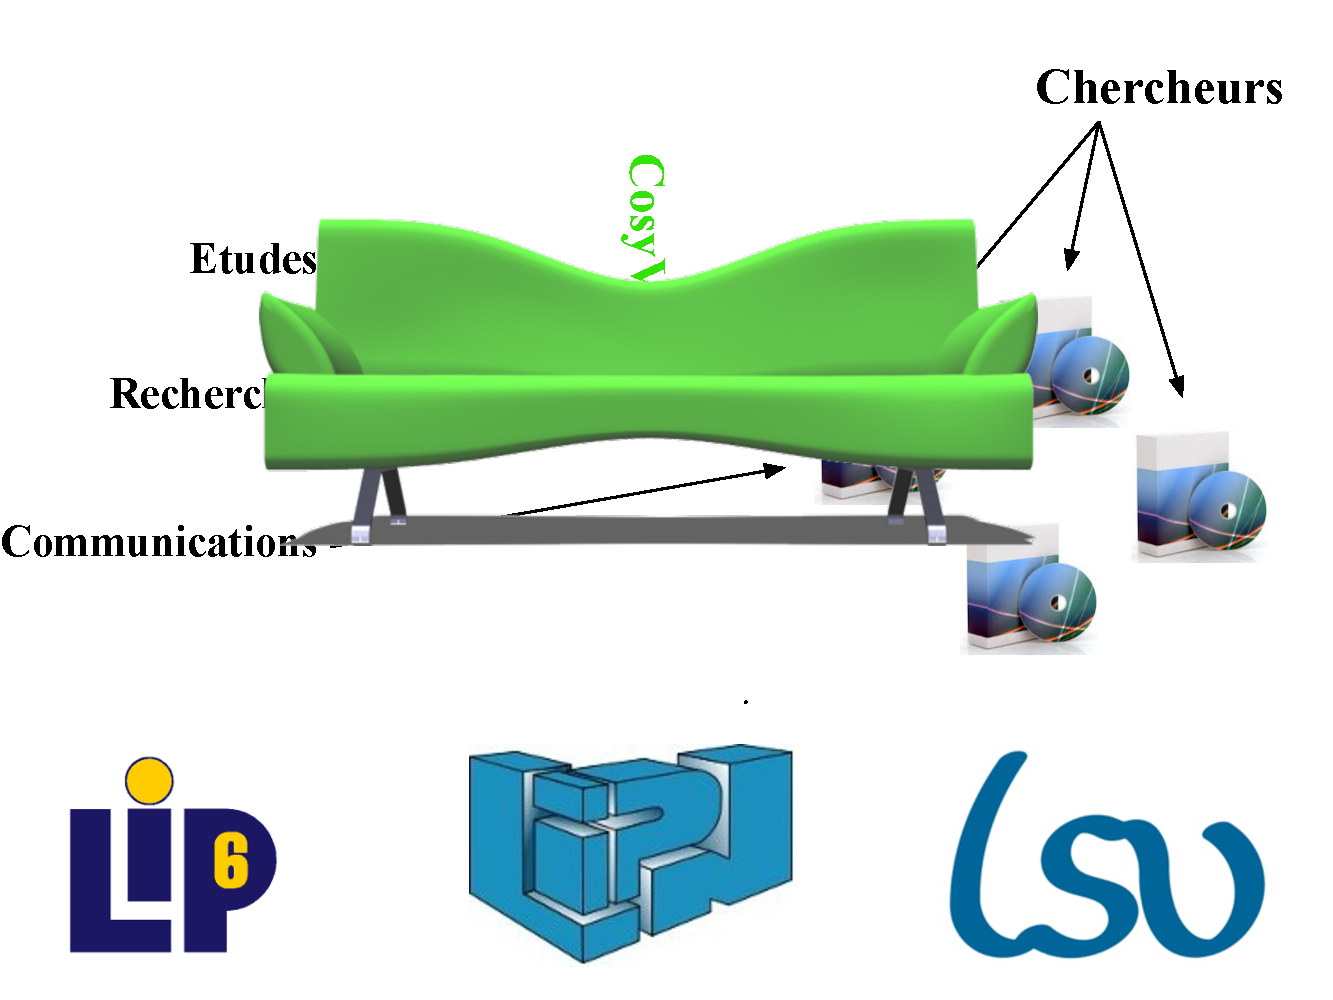
\includegraphics[width=10.5cm, height=4cm]{img/4-chercheur}};
                 \end{tikzpicture}
            }%
 
    \end{minipage}
   
   \hrule
  
  \begin{minipage}{1\textwidth}
    
         \begin{itemize}
     	    \item <3->Installer
     	    \item <4->Prise en main
	    \item <5->Format d'entrée
     	    \item <6->Format de sortie
     	    \item <7->Analyse de résultats
         \end{itemize}
   \end{minipage}
 \end{frame}
 
 \begin{frame}[c]
  \frametitle{Problématique}
  
  \begin{minipage}{1\textwidth}
  	\only <1>{%
                \begin{tikzpicture}
                      \node
                          [anchor=north]
                          at (0,0)
                          {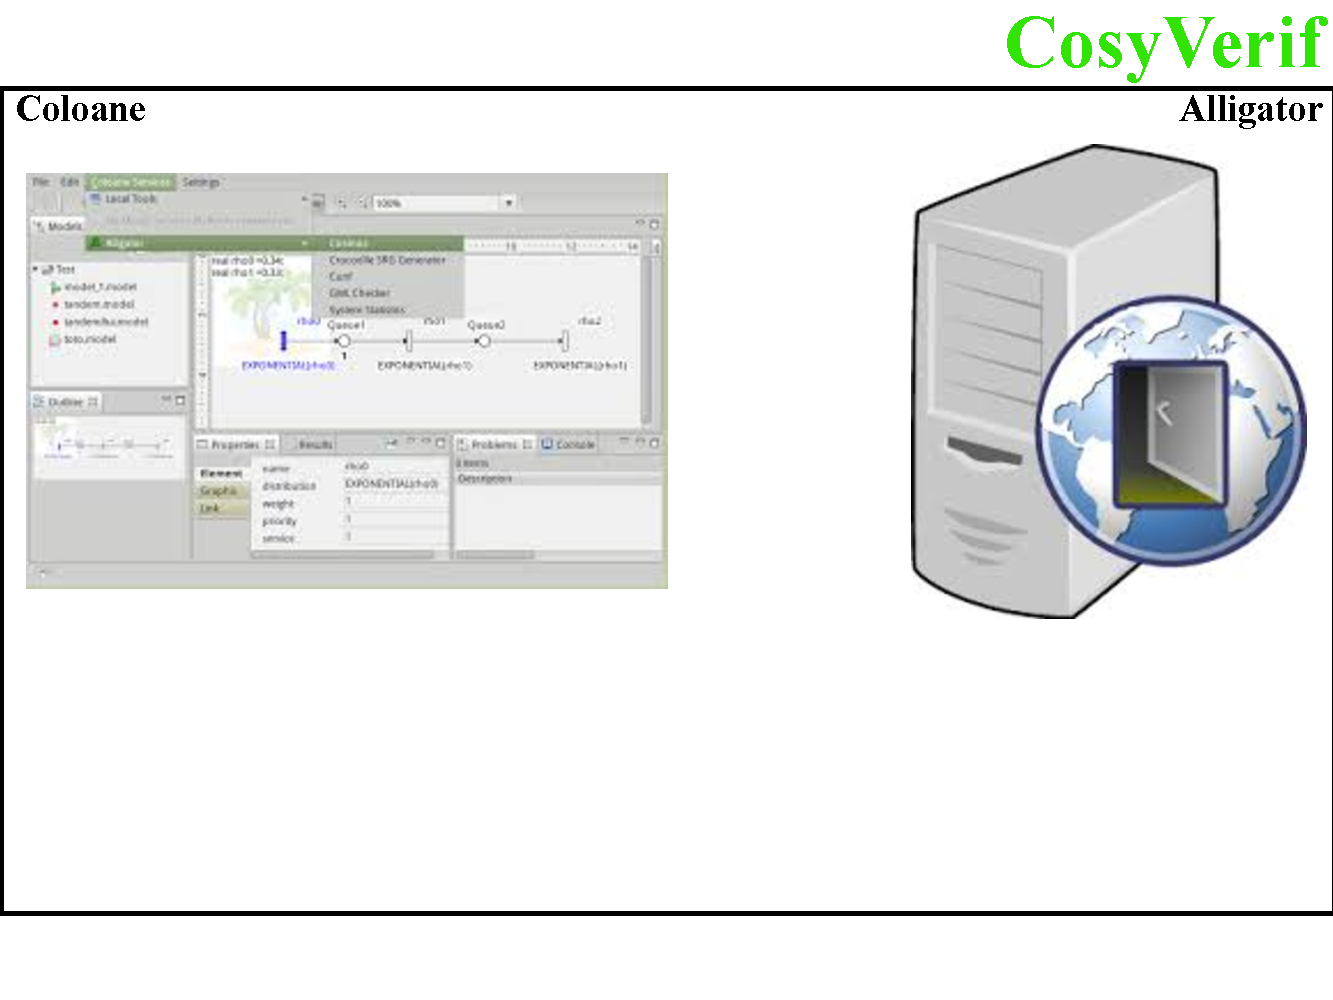
\includegraphics[width=10.5cm, height=4cm]{img/1-probleme}};
                 \end{tikzpicture}
            }%
            
            \only <2>{%
                \begin{tikzpicture}
                      \node
                          [anchor=north]
                          at (0,0)
                          {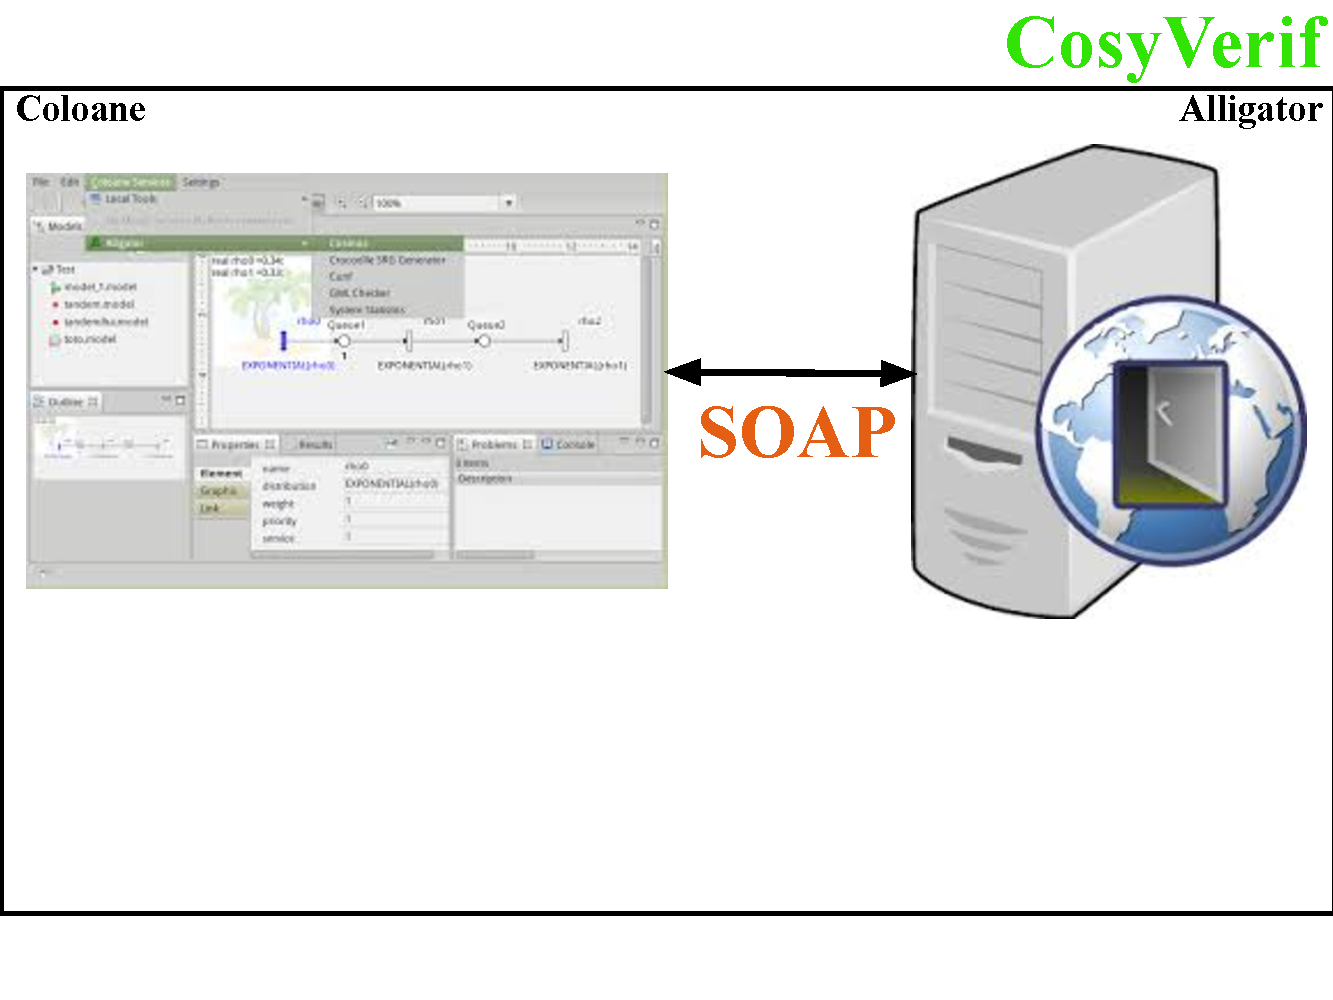
\includegraphics[width=10.5cm, height=4cm]{img/2-probleme}};
                 \end{tikzpicture}
            }%
            
            \only <3>{%
                \begin{tikzpicture}
                      \node
                          [anchor=north]
                          at (0,0)
                          {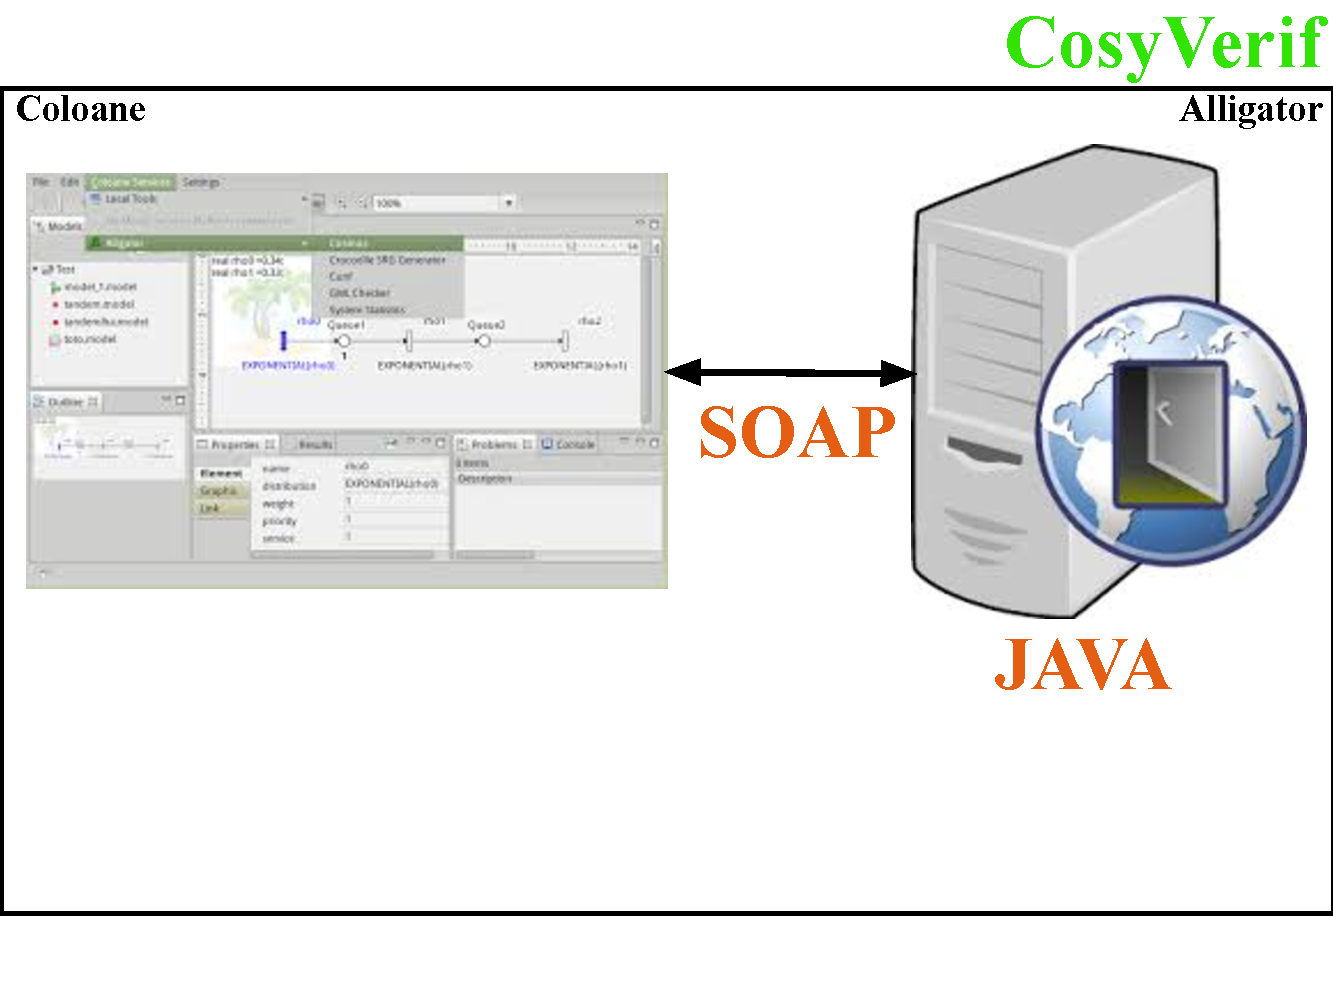
\includegraphics[width=10.5cm, height=4cm]{img/3-probleme}};
                 \end{tikzpicture}
            }%
            
            \only <4>{%
                \begin{tikzpicture}
                      \node
                          [anchor=north]
                          at (0,0)
                          {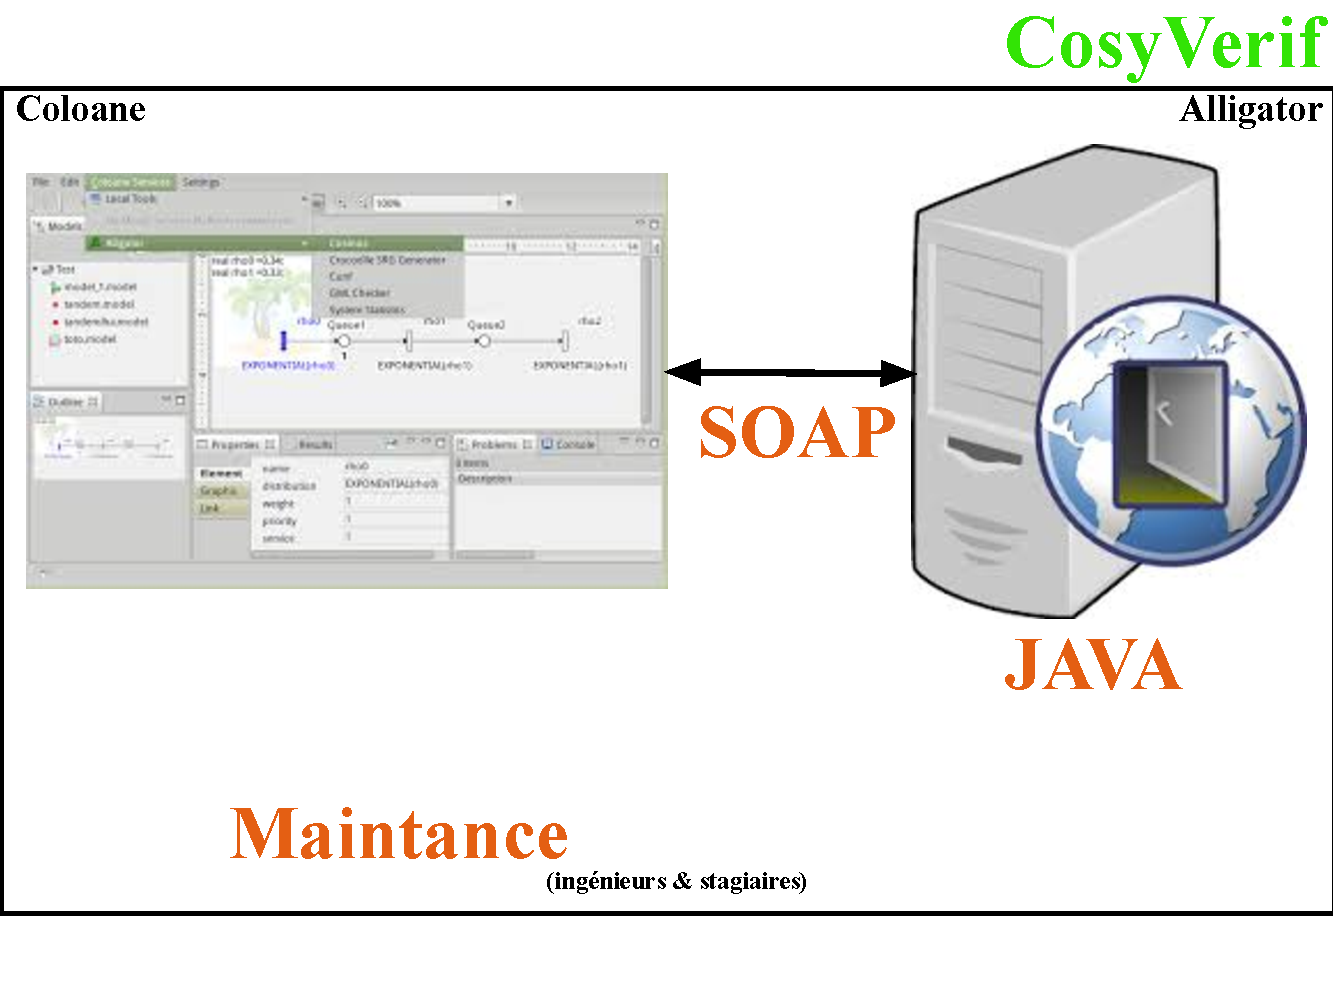
\includegraphics[width=10.5cm, height=4cm]{img/4-probleme}};
                 \end{tikzpicture}
            }%
 
    \end{minipage}
   
   \hrule
  
  \begin{minipage}{1\textwidth}
    
         \begin{itemize}
     	    \item <2-> Protocole de communication SOAP (Simple Object Access Protocol)
     	    \item <3-> Langage 
     	    \item <4->Maintenance 
         \end{itemize}
   \end{minipage}
 \end{frame}
 
 
  \begin{frame}[c]
  \frametitle{Objectifs}
  
  \begin{minipage}{1\textwidth}
  	\only <1>{%
                \begin{tikzpicture}
                      \node
                          [anchor=north]
                          at (0,0)
                          {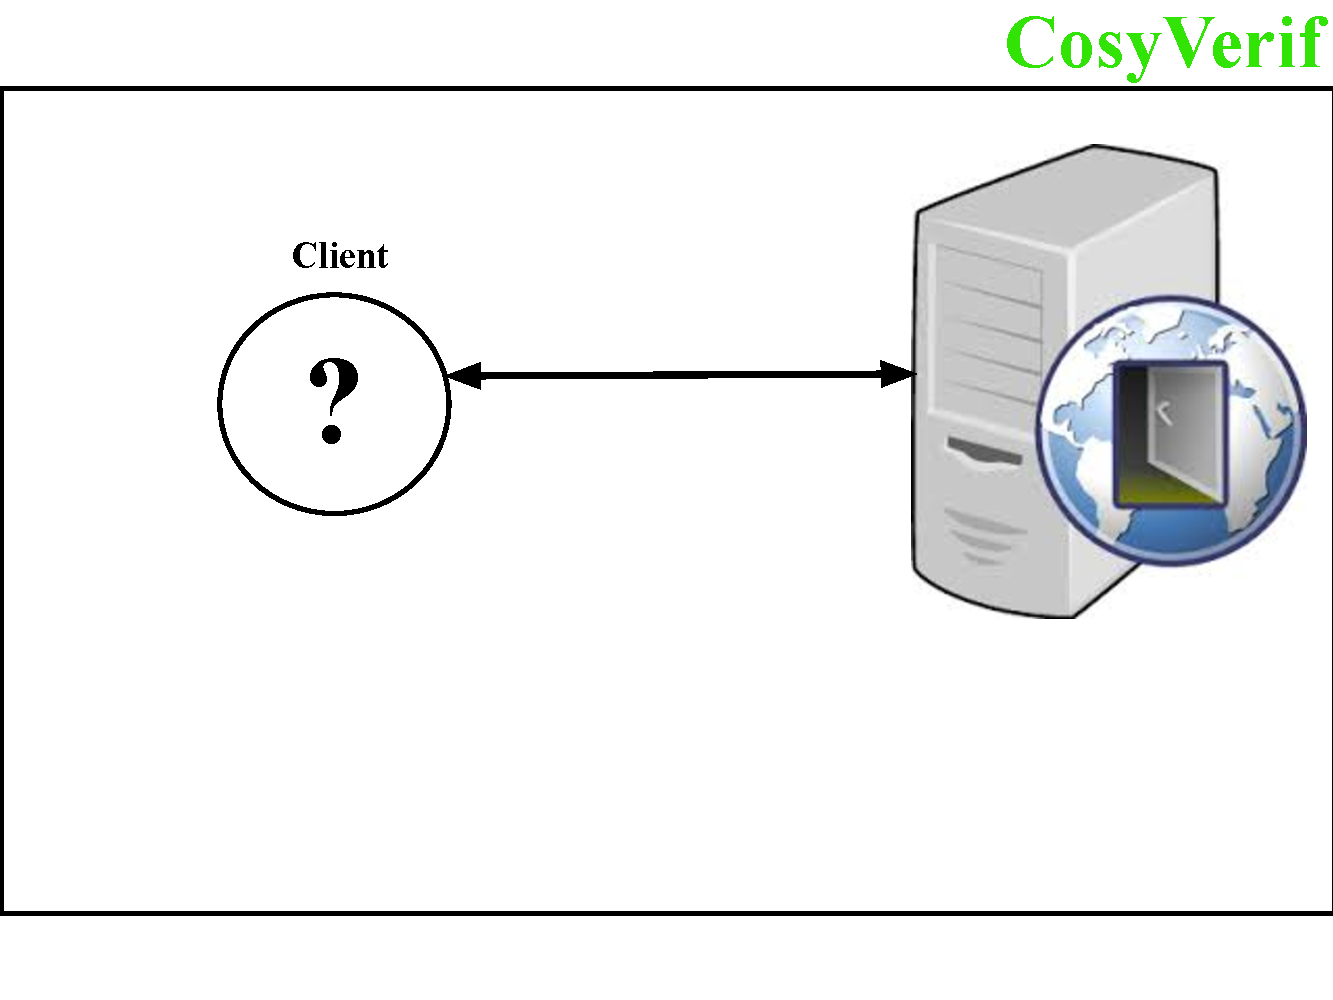
\includegraphics[width=10.5cm, height=4cm]{img/1-objectif}};
                 \end{tikzpicture}
            }%
            
            \only <2>{%
                \begin{tikzpicture}
                      \node
                          [anchor=north]
                          at (0,0)
                          {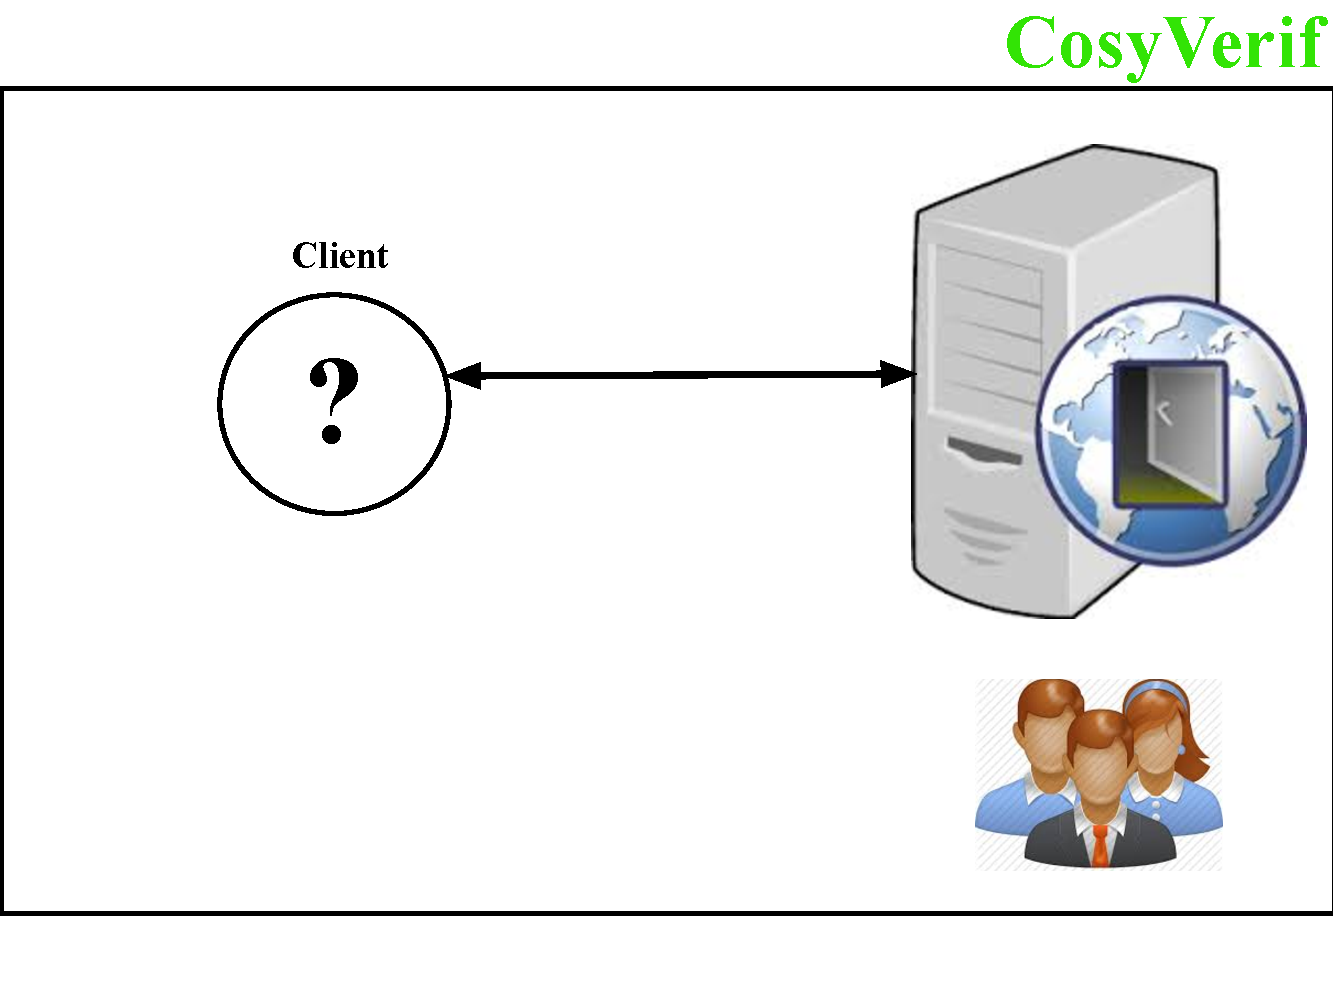
\includegraphics[width=10.5cm, height=4cm]{img/2-objectif}};
                 \end{tikzpicture}
            }%
            
            \only <3>{%
                \begin{tikzpicture}
                      \node
                          [anchor=north]
                          at (0,0)
                          {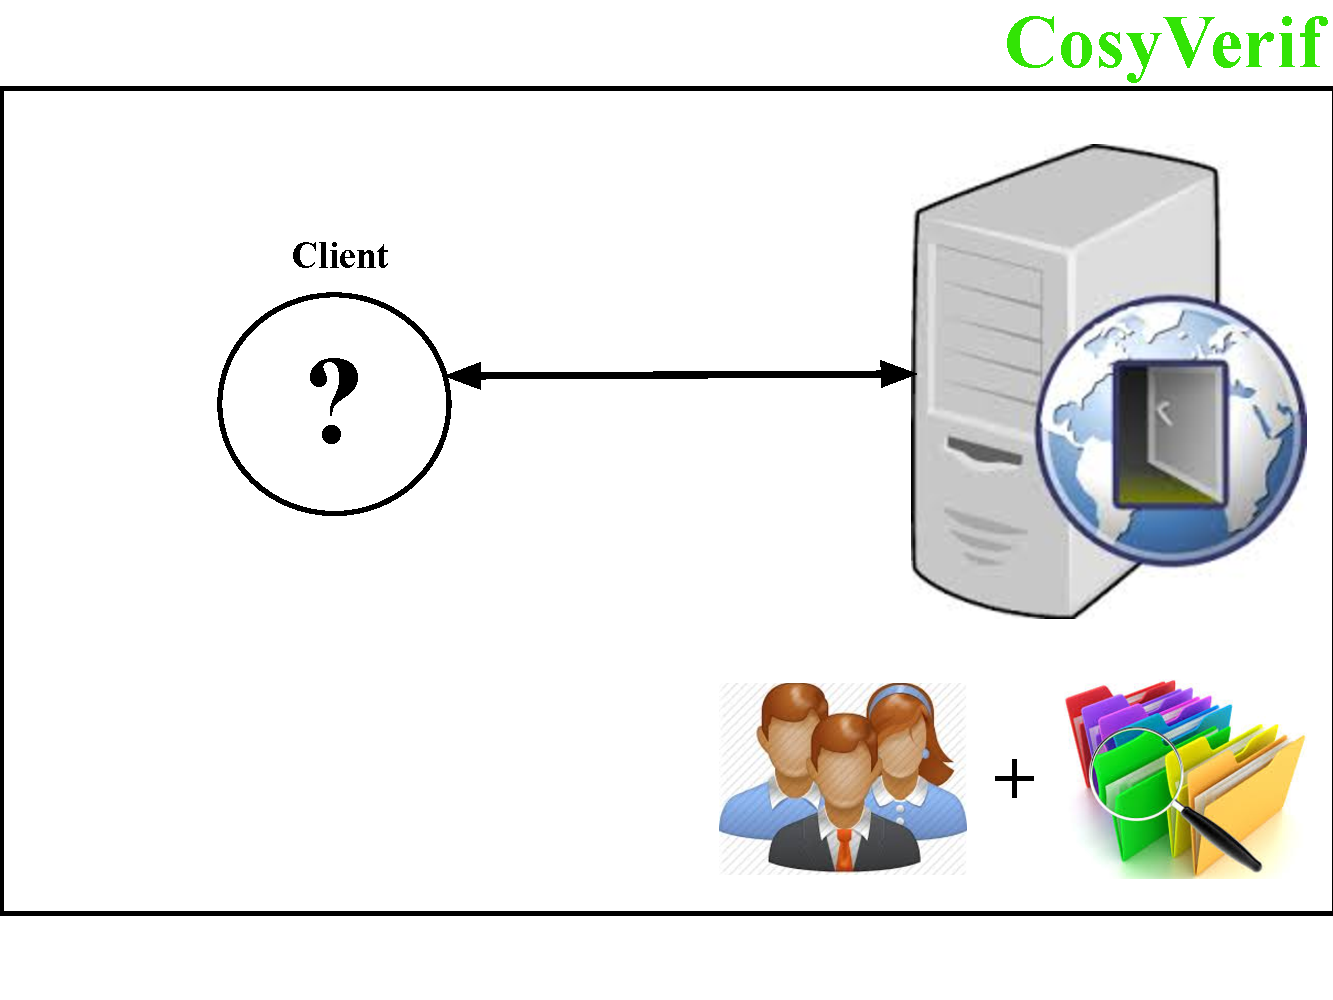
\includegraphics[width=10.5cm, height=4cm]{img/3-objectif}};
                 \end{tikzpicture}
            }%
            
            \only <4>{%
                \begin{tikzpicture}
                      \node
                          [anchor=north]
                          at (0,0)
                          {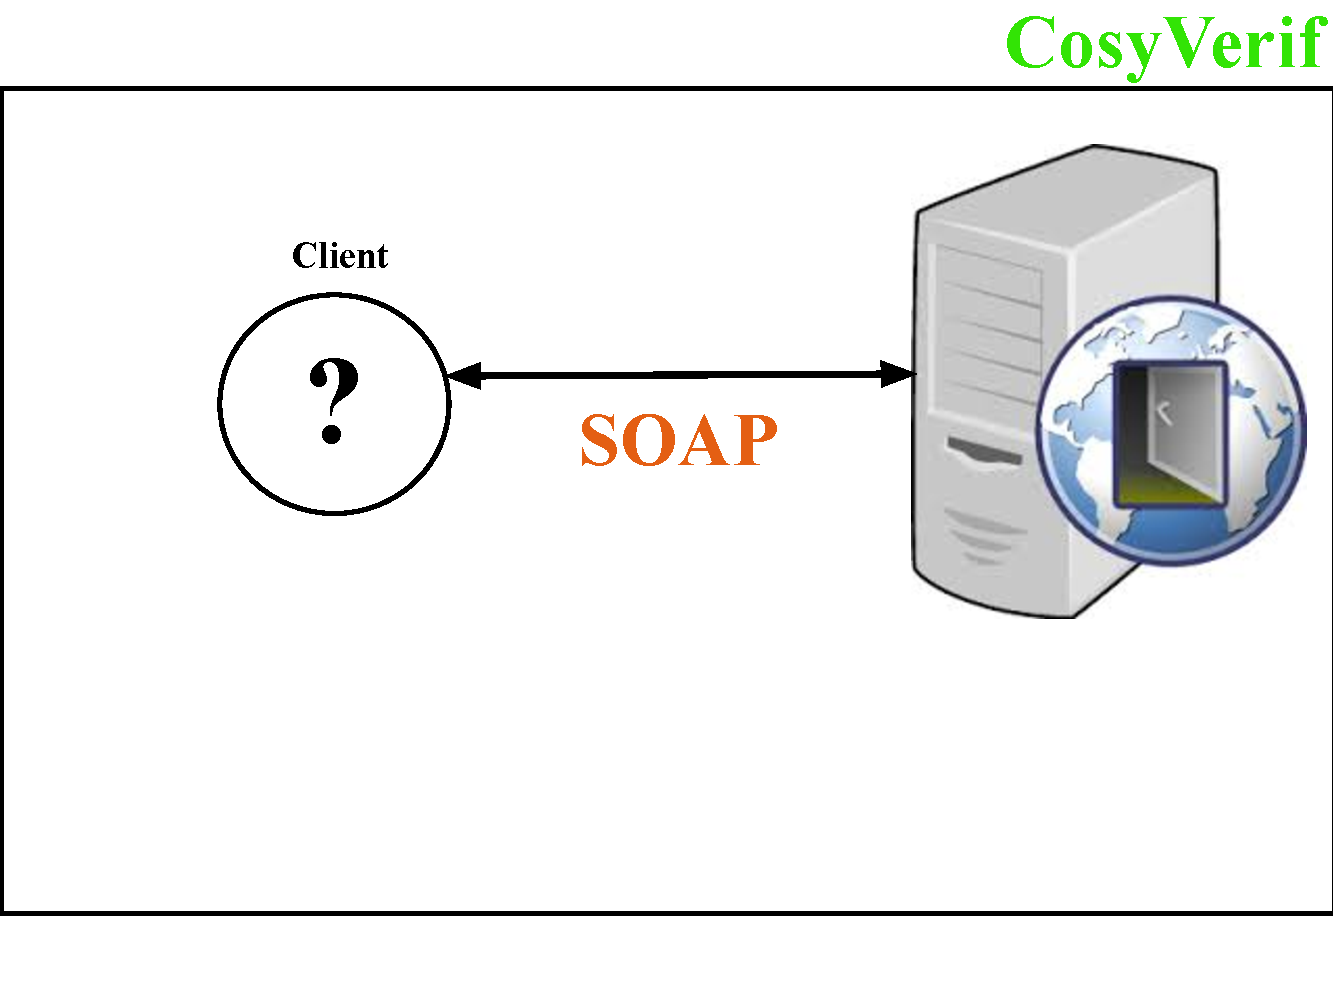
\includegraphics[width=10.5cm, height=4cm]{img/4-objectif}};
                 \end{tikzpicture}
            }%
            
            \only <5>{%
                \begin{tikzpicture}
                      \node
                          [anchor=north]
                          at (0,0)
                          {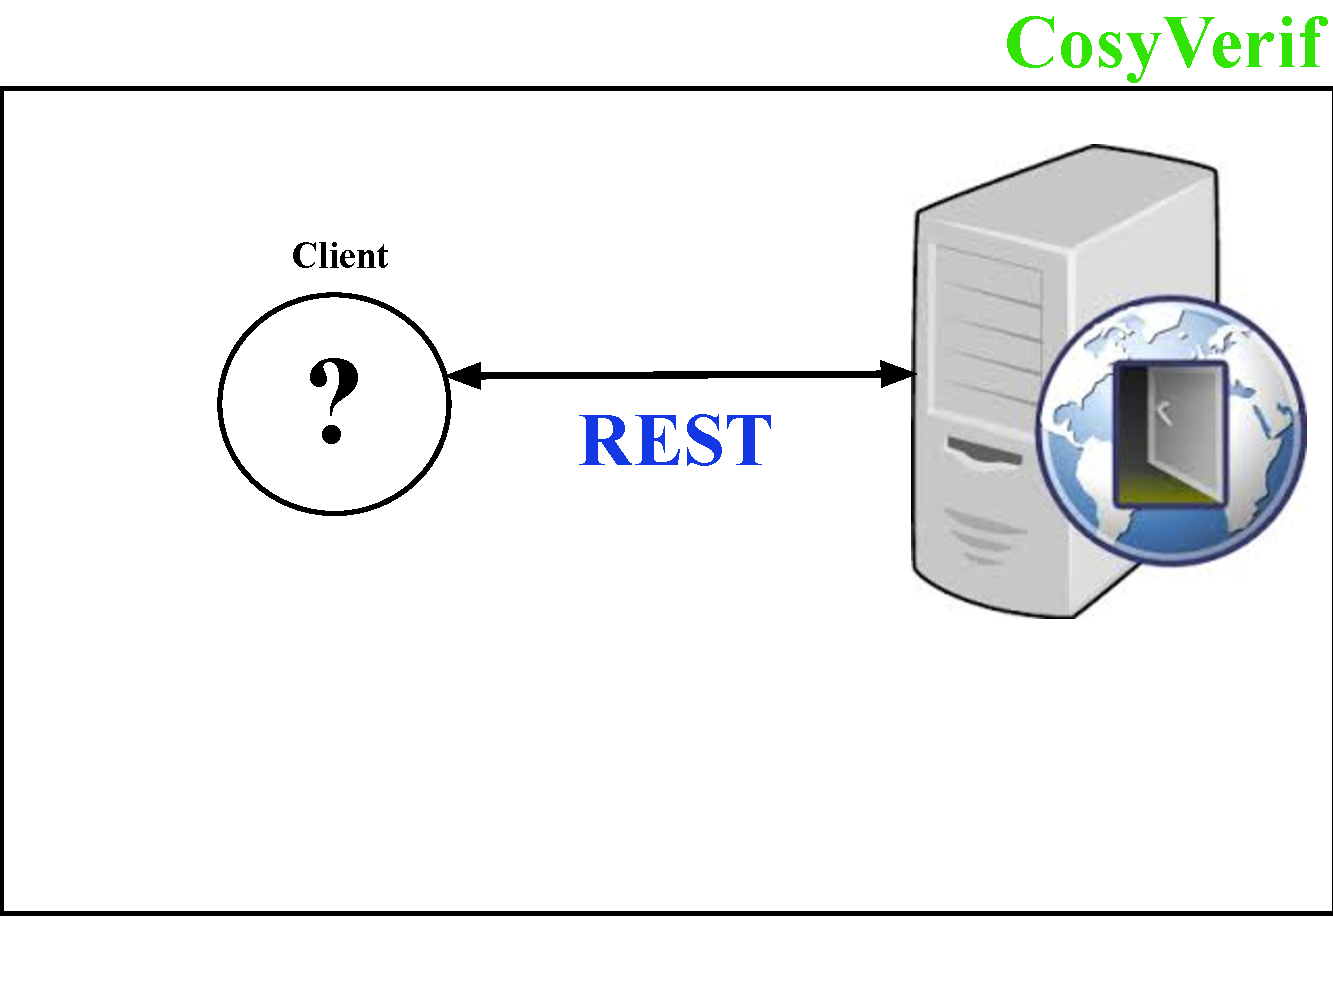
\includegraphics[width=10.5cm, height=4cm]{img/5-objectif}};
                 \end{tikzpicture}
            }%
            
            \only <6>{%
                \begin{tikzpicture}
                      \node
                          [anchor=north]
                          at (0,0)
                          {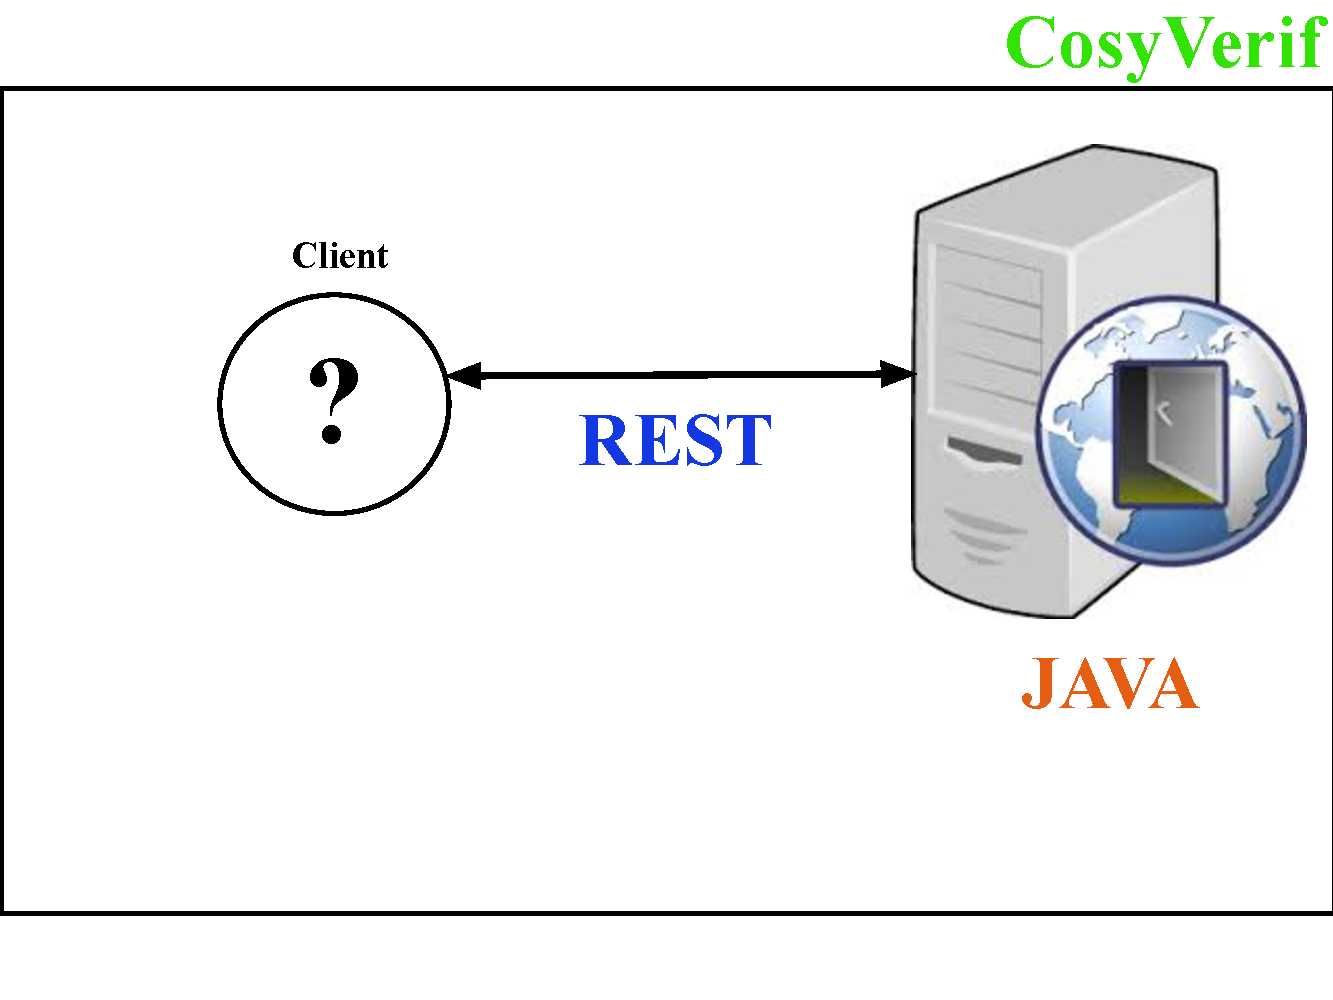
\includegraphics[width=10.5cm, height=4cm]{img/6-objectif}};
                 \end{tikzpicture}
            }%
            
            \only <7>{%
                \begin{tikzpicture}
                      \node
                          [anchor=north]
                          at (0,0)
                          {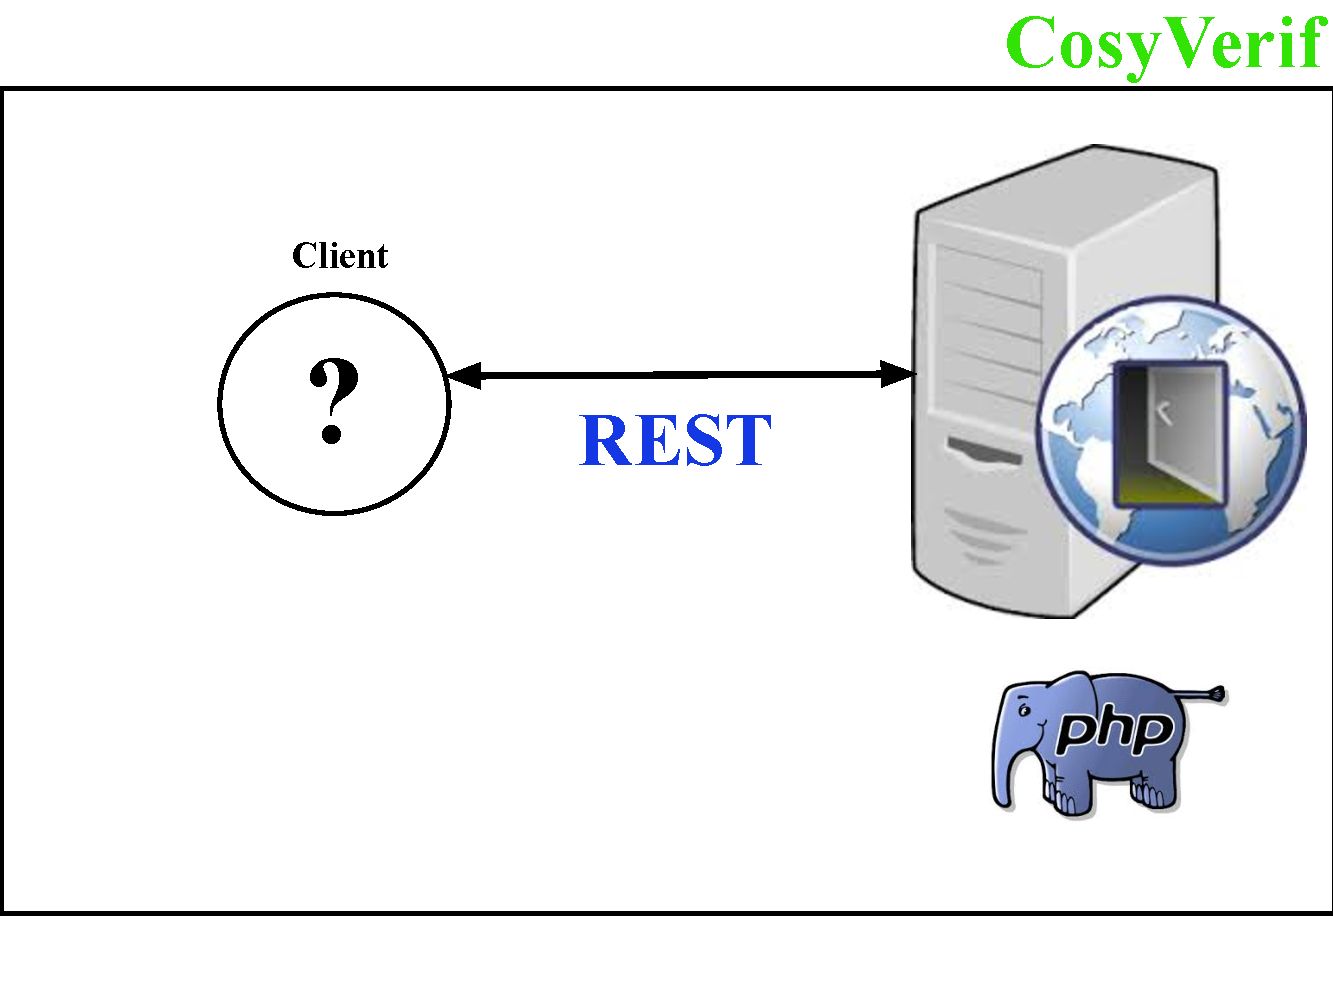
\includegraphics[width=10.5cm, height=4cm]{img/7-objectif}};
                 \end{tikzpicture}
            }%
            
            \only <8>{%
                \begin{tikzpicture}
                      \node
                          [anchor=north]
                          at (0,0)
                          {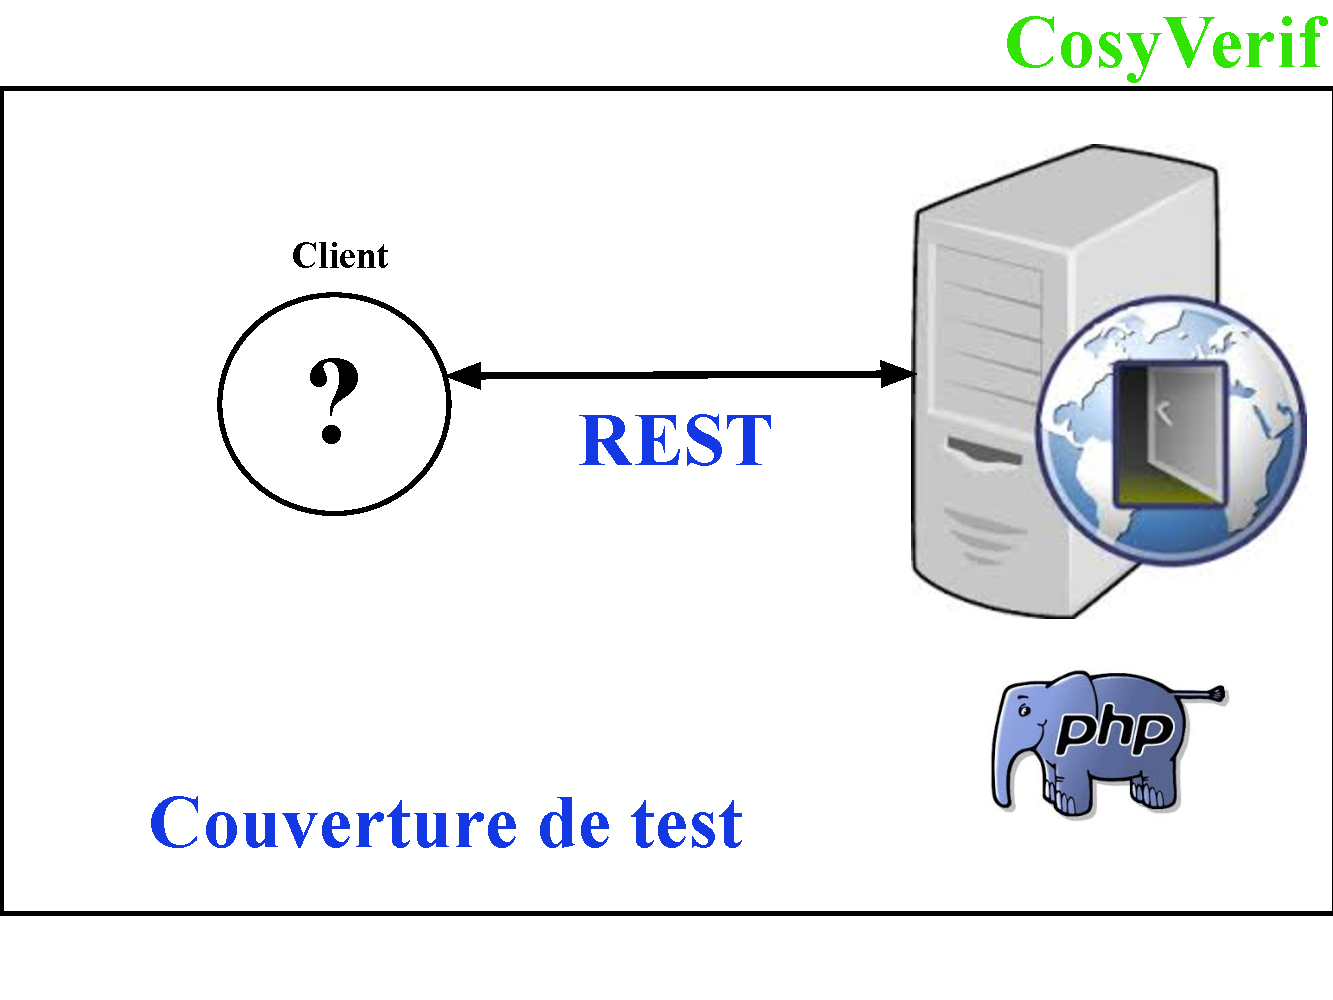
\includegraphics[width=10.5cm, height=4cm]{img/8-objectif}};
                 \end{tikzpicture}
            }%
 
    \end{minipage}
   
   \hrule
  
  \begin{minipage}{1\textwidth}
    
         \begin{itemize}
     	    \item <1-> Serveur maintenable
     	    \item <2-> Gestion des utilisateurs 
     	    \item <3-> Dépôt de modèles et de formalisms (comme PNMLWEB)
	    \item <4-> SOAP => REST (Representation State Transfert)
     	    \item <6-> JAVA => PHP 
     	    \item <8-> Test
         \end{itemize}
   \end{minipage}
 \end{frame}
 
    \begin{frame}[c]
  \frametitle{Arborescence utilisateurs}
  
  \begin{minipage}{1\textwidth}
  	\only <1-9>{%
                \begin{tikzpicture}
                      \node
                          [anchor=north]
                          at (0,0)
                          {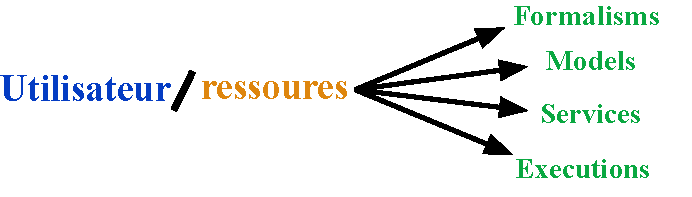
\includegraphics[width=10.5cm, height=4cm]{img/1-arbre-u}};
                 \end{tikzpicture}
            }%
            
            \only <10->{%
                \begin{tikzpicture}
                      \node
                          [anchor=north]
                          at (0,0)
                          {
\includegraphics[width=10.5cm, height=4cm]{img/2-arbre-u}};
                 \end{tikzpicture}
            }%
            
 
    \end{minipage}
   
   \hrule
  
  \begin{minipage}[t][15cm][t]{\textheight}
  
  \begin{columns}[T] % align columns
\begin{column}{.48\textwidth}
\only<2>{%
\lstinline!GET http://rest.cosyverif.org/users! \\
\lstinline!200 OK! \\
\lstinline!{ ... }!
}%
\only<3>{%
\lstinline!POST .../users/isokhona! \\
\lstinline!201 CREATED!
}%
\only<4>{%
\lstinline!POST .../users/alban! \\
\lstinline!201 CREATED!
}%

\only<5>{%
\lstinline!POST .../users/isokhona/models/model1! \\
\lstinline!201 CREATED!
}%

\only<6>{%
\lstinline!GET .../users/isokhona/models/model1! \\
\lstinline!200 OK & data!
}%

\only<7>{%
\lstinline!PUT .../users/isokhona/models/model1! \\
\lstinline!200 OK!
}%

\only<8>{%
\lstinline!DELETE .../users/isokhona/models/model1! \\
\lstinline!204 NO CONTENT!
}%

\only<9>{%
\lstinline!GET .../users/isokhona/models/model1! \\
\lstinline!410 GONE!
}%

\end{column}%
\hfill%
\begin{column}{.48\textwidth}
% http://www.texample.net/tikz/examples/filesystem-tree/
\tikzstyle{every node}=[draw=black,thick,anchor=west,minimum width=2cm,minimum height=2em]
\tikzstyle{selected}=[draw=red,fill=red!30]
\tikzstyle{optional}=[dashed,fill=gray!50]
\scriptsize
\begin{tikzpicture}[
every node={draw=black,thick,anchor=west},
selected={draw=red,fill=red!30},
grow via three points={one child at (-.5,-0.7) and
two children at (-.5,-0.7) and (-.5,-1.4)},
edge from parent path={(\tikzparentnode.south west) |- (\tikzchildnode.west)}]
\only<2->{
\node {/}
child { node {users} };
}
\end{tikzpicture}
\end{column}%
\end{columns}
    
   \end{minipage}
 \end{frame}
 
     \begin{frame}[c]
  \frametitle{Arborescence Projets}
  
  \begin{minipage}{1\textwidth}
  	\only <1>{%
                \begin{tikzpicture}
                      \node
                          [anchor=north]
                          at (0,0)
                          {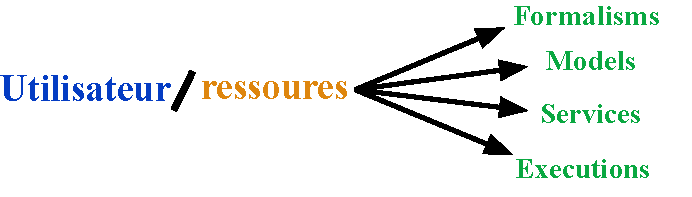
\includegraphics[width=10.5cm, height=4cm]{img/1-arbre-u}};
                 \end{tikzpicture}
            }%
            
            \only <2>{%
                \begin{tikzpicture}
                      \node
                          [anchor=north]
                          at (0,0)
                          {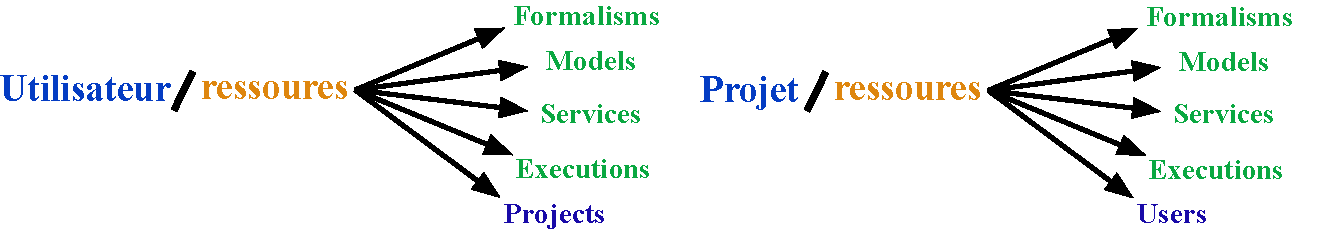
\includegraphics[width=10.5cm, height=4cm]{img/1-arbre-p}};
                 \end{tikzpicture}
            }%
            
            \only <3->{%
                \begin{tikzpicture}
                      \node
                          [anchor=north]
                          at (0,0)
                          {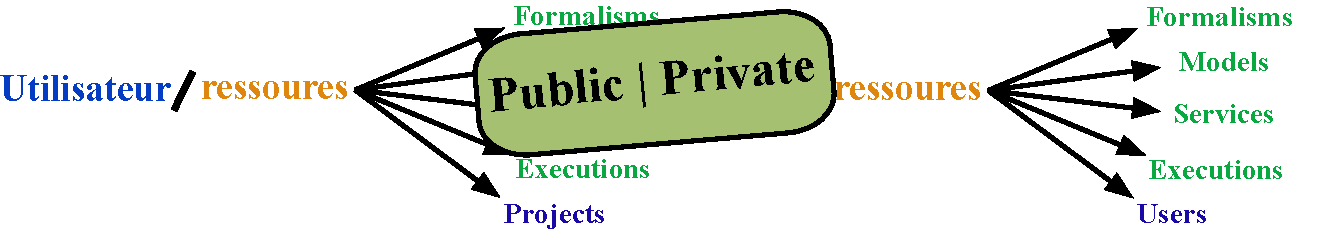
\includegraphics[width=10.5cm, height=4cm]{img/2-arbre-p}};
                 \end{tikzpicture}
            }%
            
 
    \end{minipage}
   
   \hrule
  
  \begin{minipage}[t][15cm][t]{\textheight}
  
  \begin{columns}[T] % align columns
\begin{column}{.48\textwidth}
\only<2->{%
\lstinline!GET http://rest.cosyverif.org/users! \\
\lstinline!200 OK! \\
\lstinline!{ ... }!
}%

\end{column}%
\hfill%
\begin{column}{.48\textwidth}
% http://www.texample.net/tikz/examples/filesystem-tree/
\tikzstyle{every node}=[draw=black,thick,anchor=west,minimum width=2cm,minimum height=2em]
\tikzstyle{selected}=[draw=red,fill=red!30]
\tikzstyle{optional}=[dashed,fill=gray!50]
\scriptsize
\begin{tikzpicture}[
every node={draw=black,thick,anchor=west},
selected={draw=red,fill=red!30},
grow via three points={one child at (-.5,-0.7) and
two children at (-.5,-0.7) and (-.5,-1.4)},
edge from parent path={(\tikzparentnode.south west) |- (\tikzchildnode.west)}]
\only<2->{
\node {/}
child { node {projects} }
child { node {users} };
}
\end{tikzpicture}
\end{column}%
\end{columns}
    
   \end{minipage}
 \end{frame}
 
 
\begin{frame}[c]
  \frametitle{Implémentation}
  
  \begin{minipage}{1\textwidth}
  	\only <1>{%
                \begin{tikzpicture}
                      \node
                          [anchor=north]
                          at (0,0)
                          {
\includegraphics[width=10.5cm, height=4cm]{img/1-implementation}};
                 \end{tikzpicture}
            }%
            
            \only <2->{%
                \begin{tikzpicture}
                      \node
                          [anchor=north]
                          at (0,0)
                          {
\includegraphics[width=10.5cm, height=4cm]{img/2-implementation}};
                 \end{tikzpicture}
            }%

             
    \end{minipage}
   
   \hrule
  
  \begin{minipage}{1\textwidth}
    
         \begin{itemize}
     	    \item <1-> Technologies
     	    \item <2-> Test
         \end{itemize}
   \end{minipage}
 \end{frame}
 
 
\begin{frame}[c]

\begin{center}

\par
\Huge Perspectives \& Conclusion

\end{center}
  
\end{frame}

\begin{frame}[c]
  \frametitle{Problématique/Objectif}
  
  \begin{minipage}{1\textwidth}
  	\only <1>{%
                \begin{tikzpicture}
                      \node
                          [anchor=north]
                          at (0,0)
                          {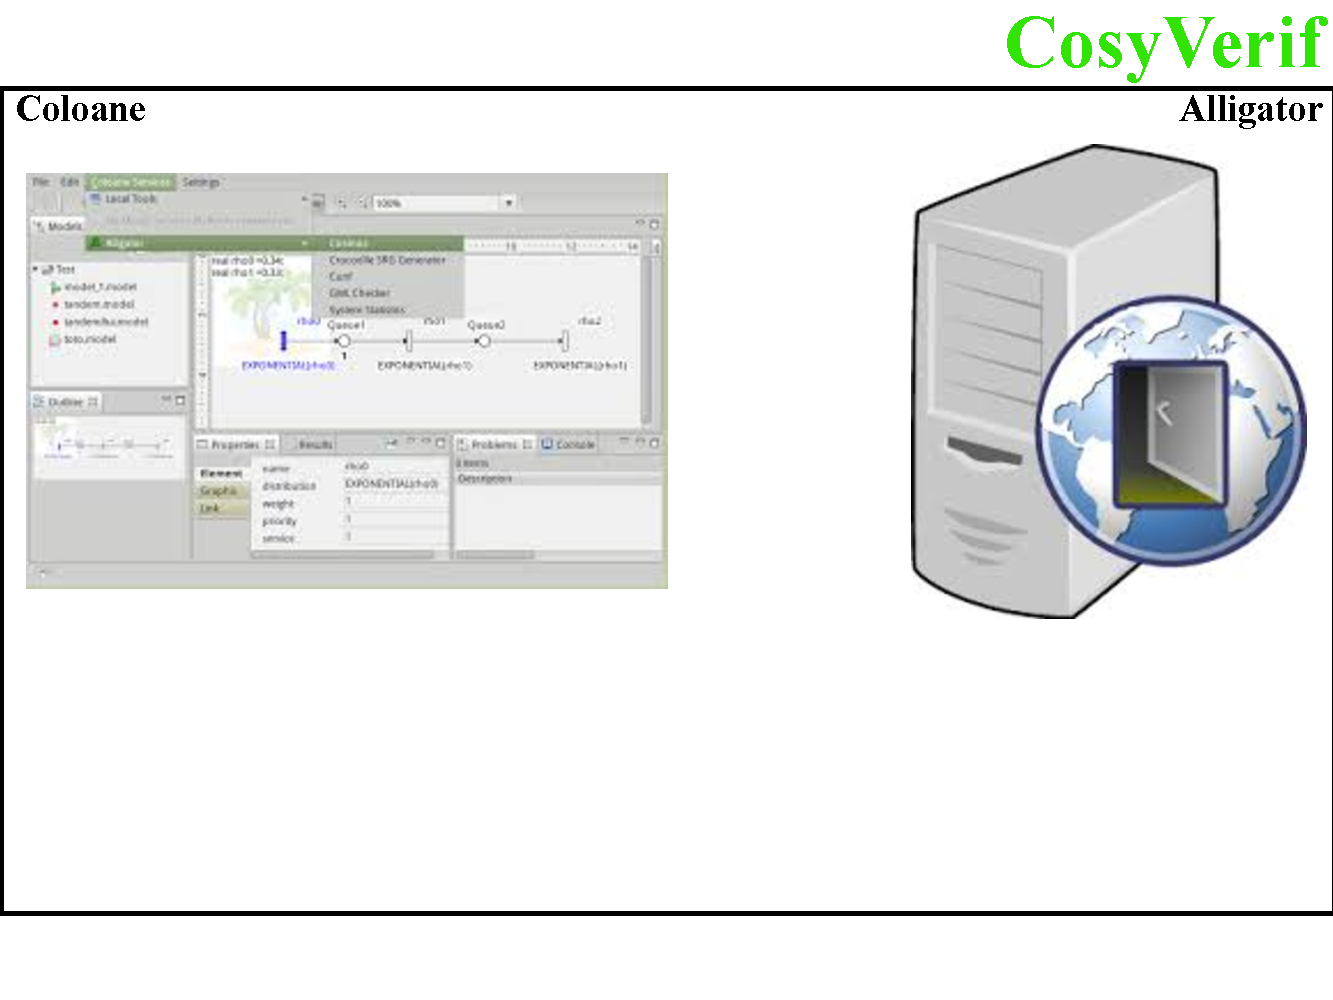
\includegraphics[width=10.5cm, height=4cm]{img/1-probleme}};
                 \end{tikzpicture}
            }%
            
            \only <2->{%
                \begin{tikzpicture}
                      \node
                          [anchor=north]
                          at (0,0)
                          {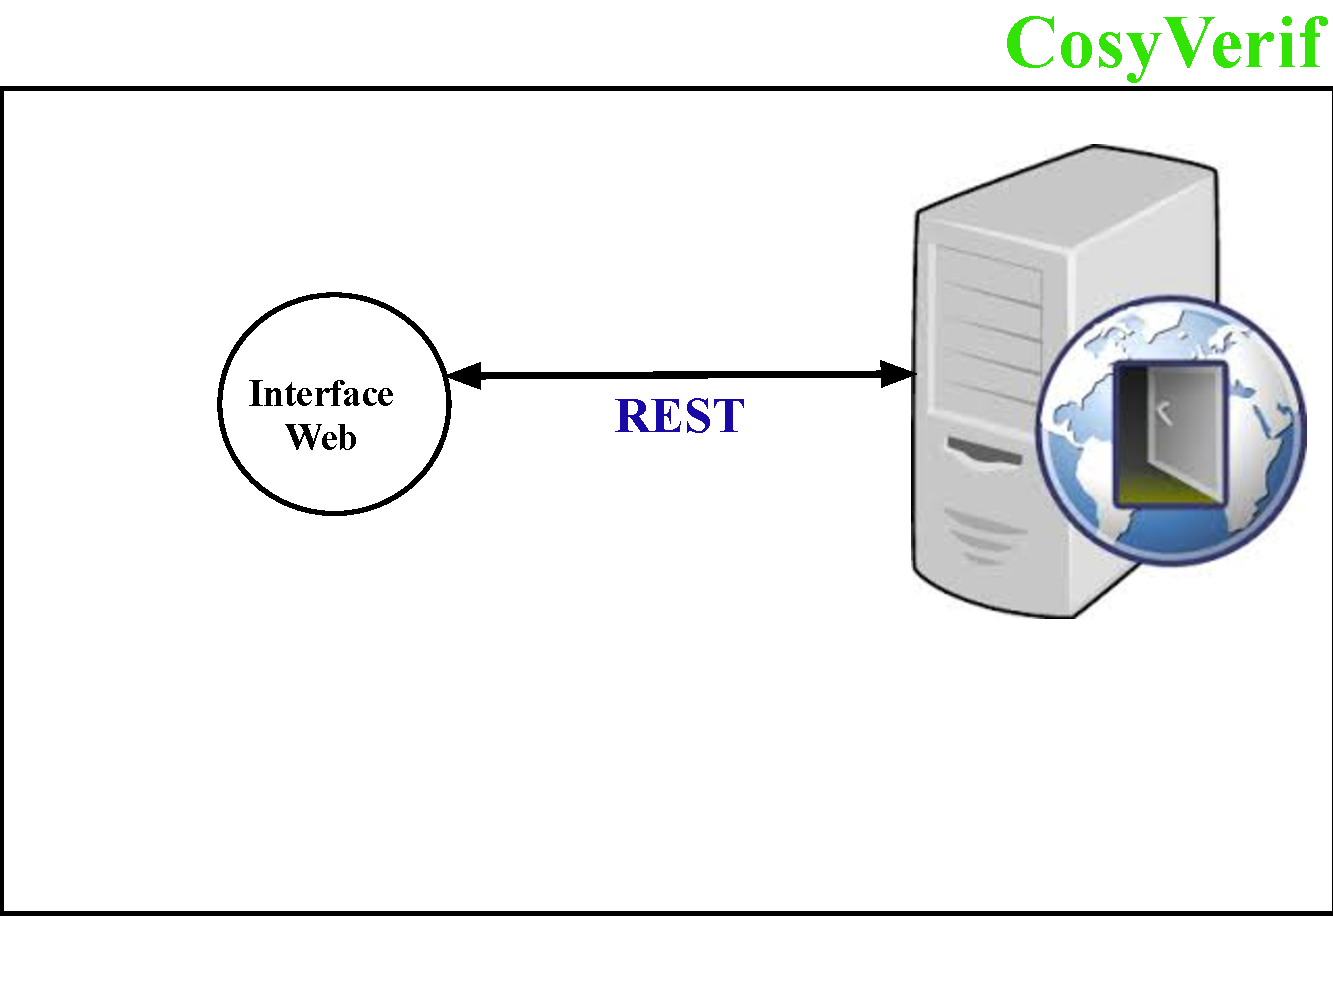
\includegraphics[width=10.5cm, height=4cm]{img/1-client}};
                 \end{tikzpicture}
            }%

             
    \end{minipage}
   
   \hrule
  
  \begin{minipage}{1\textwidth}
    
         \begin{itemize}
     	    \item <1-> Maintenance
     	    \item <1-> Fonctionnalités
	    \item <1-> Evolution
	    \item <2-> Nouvelle interface web
         \end{itemize}
   \end{minipage}
 \end{frame}
 
 
\begin{frame}[c]
  \frametitle{Interface web}
 
 \begin{columns}[T] % align columns
\begin{column}{.25\textwidth}
\only<1-2>{%
\textsf{Create user}
}%

\only<3>{%
\textsf{Create resource}
}%


\only<4>{%
\textsf{Create project}
}%

\only<5>{%
\textsf{Create invitation}
}%

\only<6>{%
\textsf{Search}
}%

\end{column}%
\hfill%
\begin{column}{.81\textwidth}

	\only <1>{%
                \begin{tikzpicture}
                      \node
                          [anchor=north]
                          at (0,0)
                          {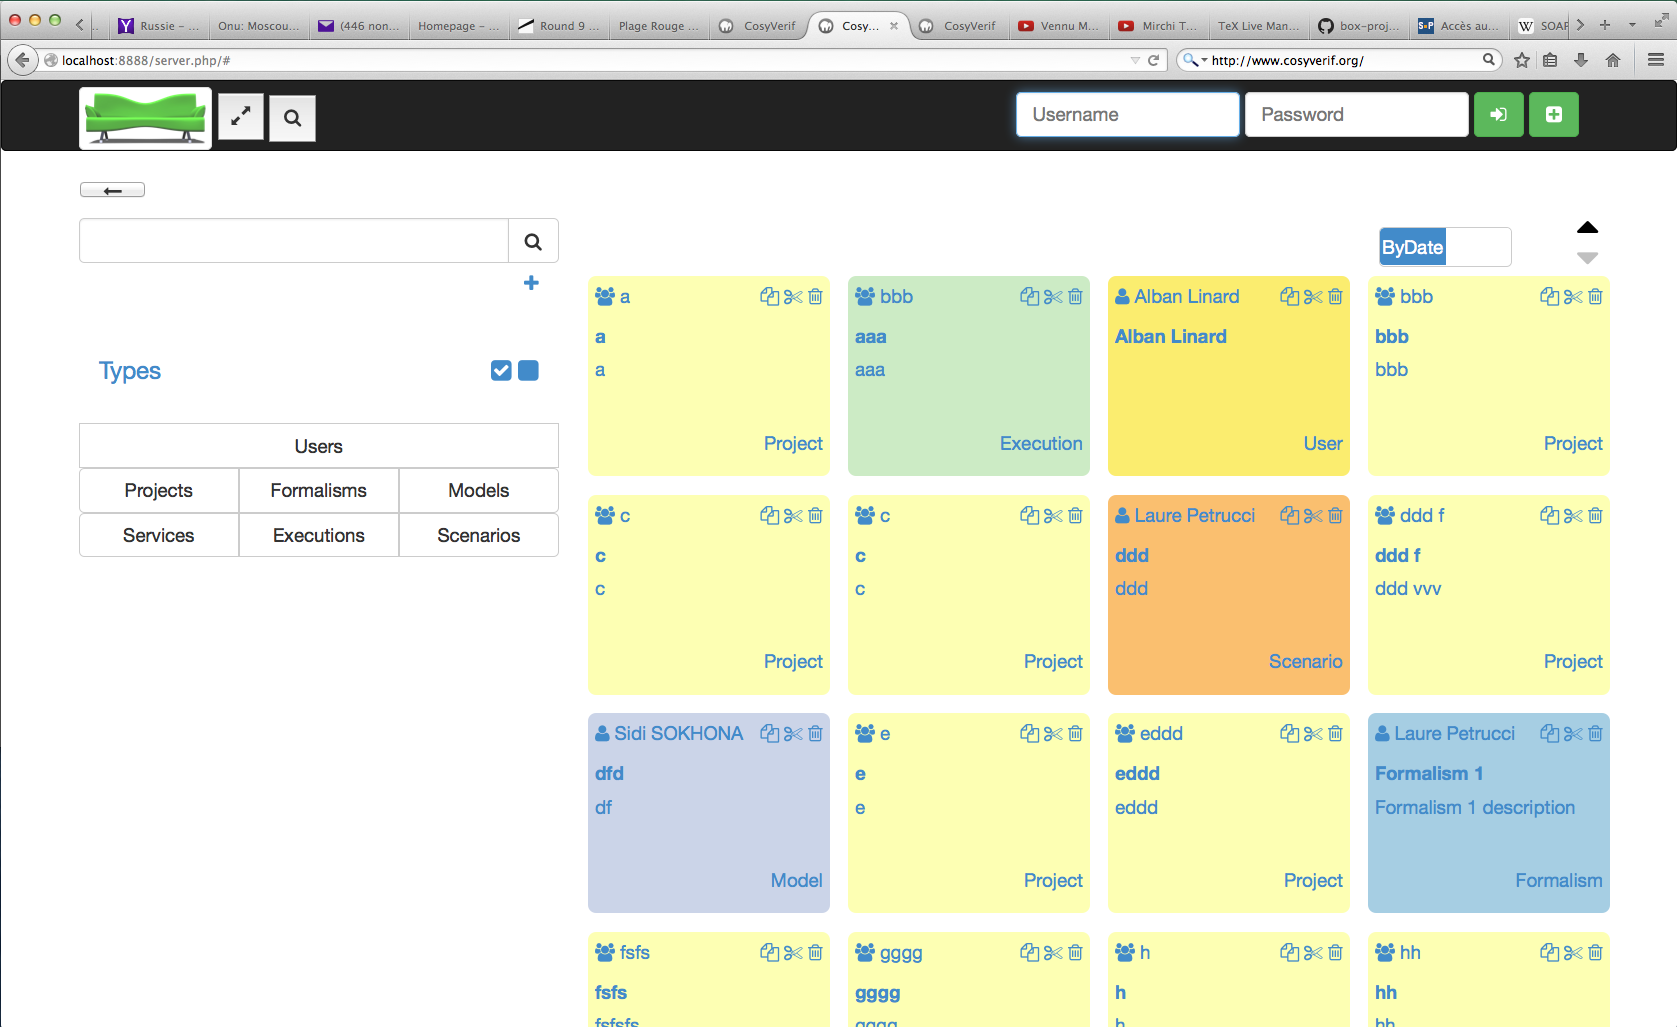
\includegraphics[width=8cm, height=10cm]{img/1-ecran-create-user}};
                 \end{tikzpicture}
            }%
            
            \only <2>{%
                \begin{tikzpicture}
                      \node
                          [anchor=north]
                          at (0,0)
                          {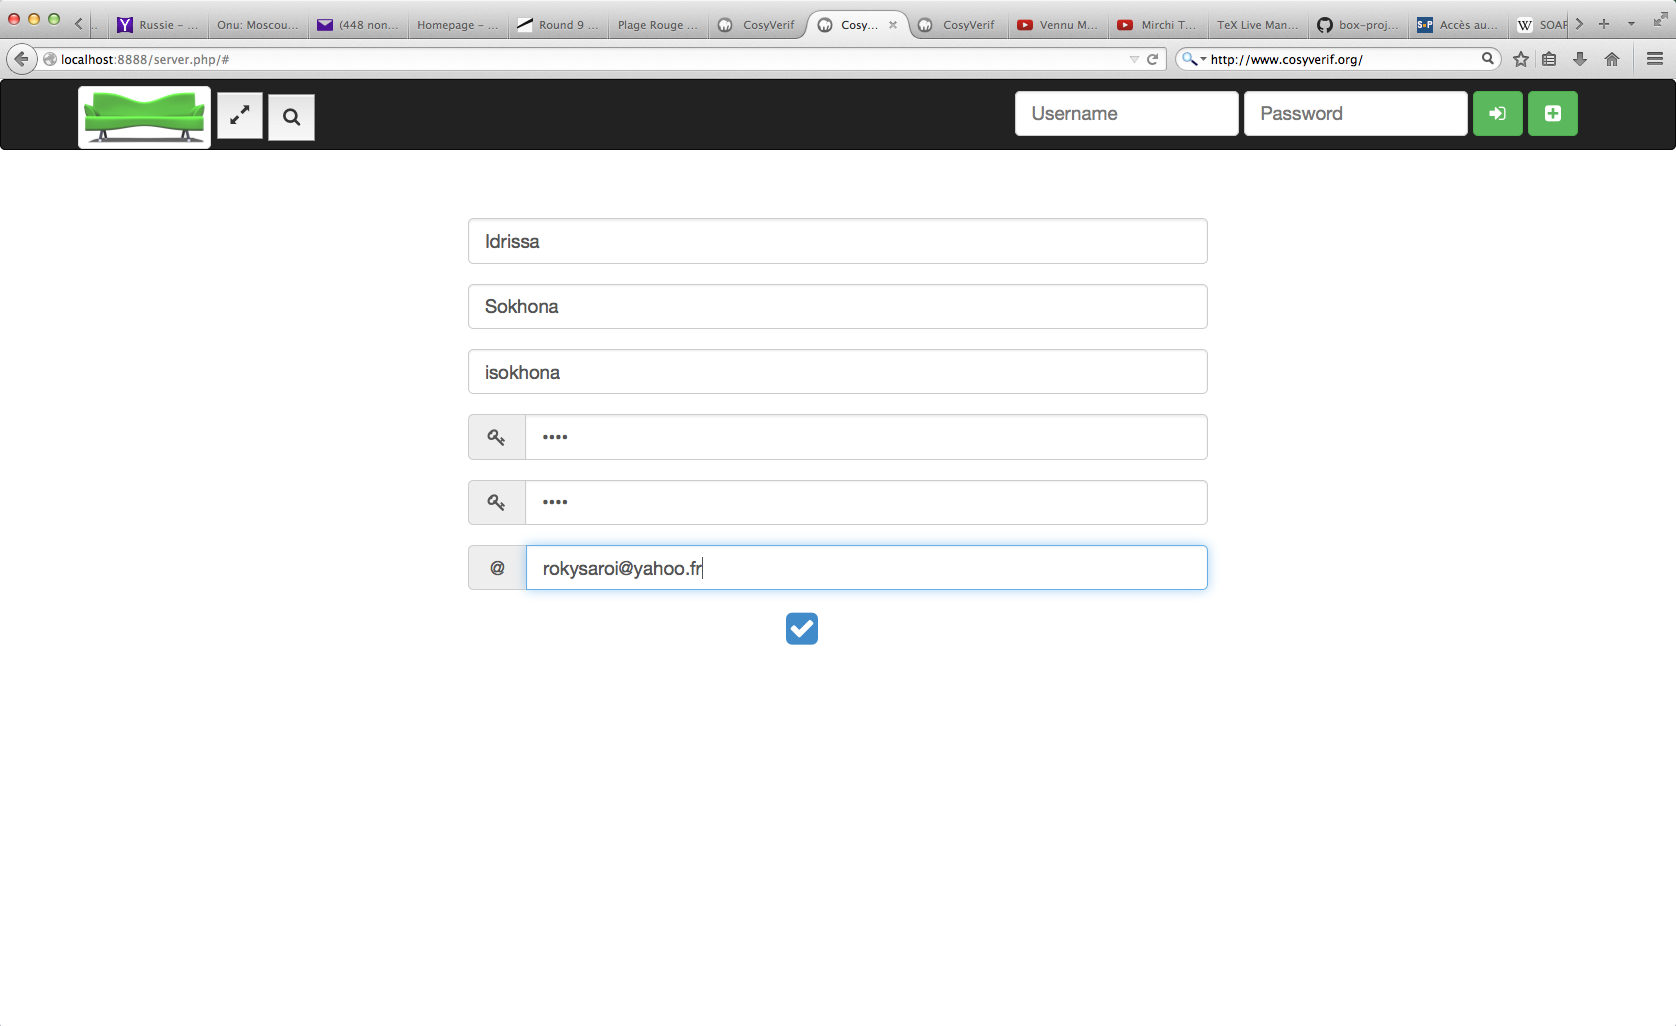
\includegraphics[width=8cm, height=10cm]{img/2-ecran-create-user}};
                 \end{tikzpicture}
            }%
\end{column}%
\end{columns}
 
  
\end{frame}

\begin{frame}[c]
  \frametitle{Implémentation}
  
  \begin{minipage}{1\textwidth}
  	\only <1->{%
                \begin{tikzpicture}
                      \node
                          [anchor=north]
                          at (0,0)
                          {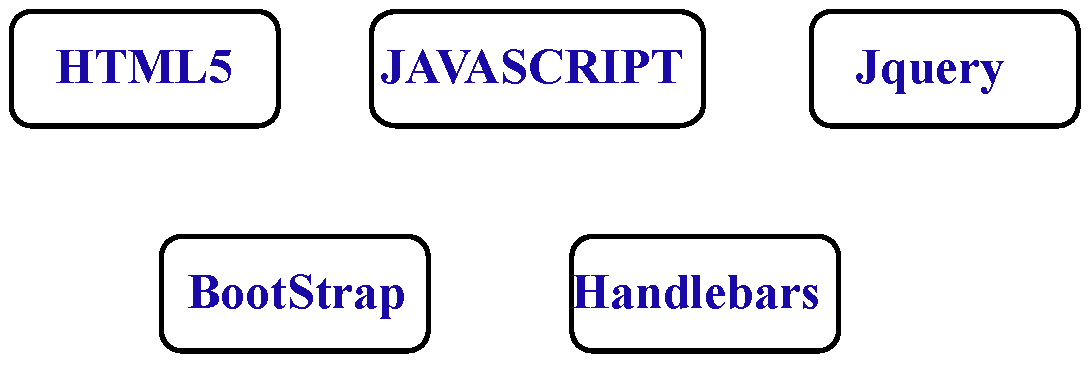
\includegraphics[width=10.5cm, height=4cm]{img/1-implementation-client}};
                 \end{tikzpicture}
            }%
            
    \end{minipage}
   
   \hrule
  
  \begin{minipage}{1\textwidth}
    
         \begin{itemize}
     	    \item <1-> Technologies
         \end{itemize}
   \end{minipage}
 \end{frame}
 
 \begin{frame}[c]

\par
\Huge Perspectives \& Conclusion

\end{center}
  
\end{frame}

\begin{frame}[c]
  \frametitle{Bilan}
  
  \begin{minipage}{1\textwidth}
  	
\begin {center}
	\par
	\Huge Bilan
\end{center}
             
    \end{minipage}
   
   \hrule
  
  \begin{minipage}{1\textwidth}
    
         \begin{itemize}
     	    \item <1-> Serveur
     	    \item <2-> Interface web
	    \item <3-> Personnel
         \end{itemize}
   \end{minipage}
\end{frame}

\begin{frame}[c]

\begin{center}

\par
\Huge Question ?

\end{center}
\end{frame}

\end{document}
